\chapter{Funktionstest/Validierung}\label{chap:Funktionstest}
\thispagestyle{standard}
\pagestyle{standard}
\lfoot{\small Refik Kerimi}

\section{Ausgangsbedingung und Ausgrenzung}
Getestet wurden die in Kapitel \ref{chab:FeaturesundMerkmale} und \ref{chap:Implementierung} beschriebenen PWA-Features. Dies wurde zum einen über die DevTools vom Chrome Browser sowie über das Chrome PlugIN Lighthouse getestet. 
Als mobiles Testgerät wurde das Nexus X5 mit der Android 8.1.0 Software verwendet.  
Weiters kann der Emulator von Android Studio verwendet werden um den Test ohne Androidgerät darzustellen. Die Applikation selbst wurde hier nicht behandelt.
 
\section{Testen auf Mobilen Geräten und Android Studio Emulator}
Um auf auf dem Mobilen Smartphone testen zu können muss der Developer Modus auf dem Gerät eingeschaltet werden. Dies wird durch das Aktivieren der Entwicklertools und das Freischalten der USB-Debugging Funktion wie in Abbildung \ref{fig:DevToolsAndorid} und \ref{fig:DevToolsChrome} zu sehen ist erreicht. 

\begin{figure}[h]
	\centering
	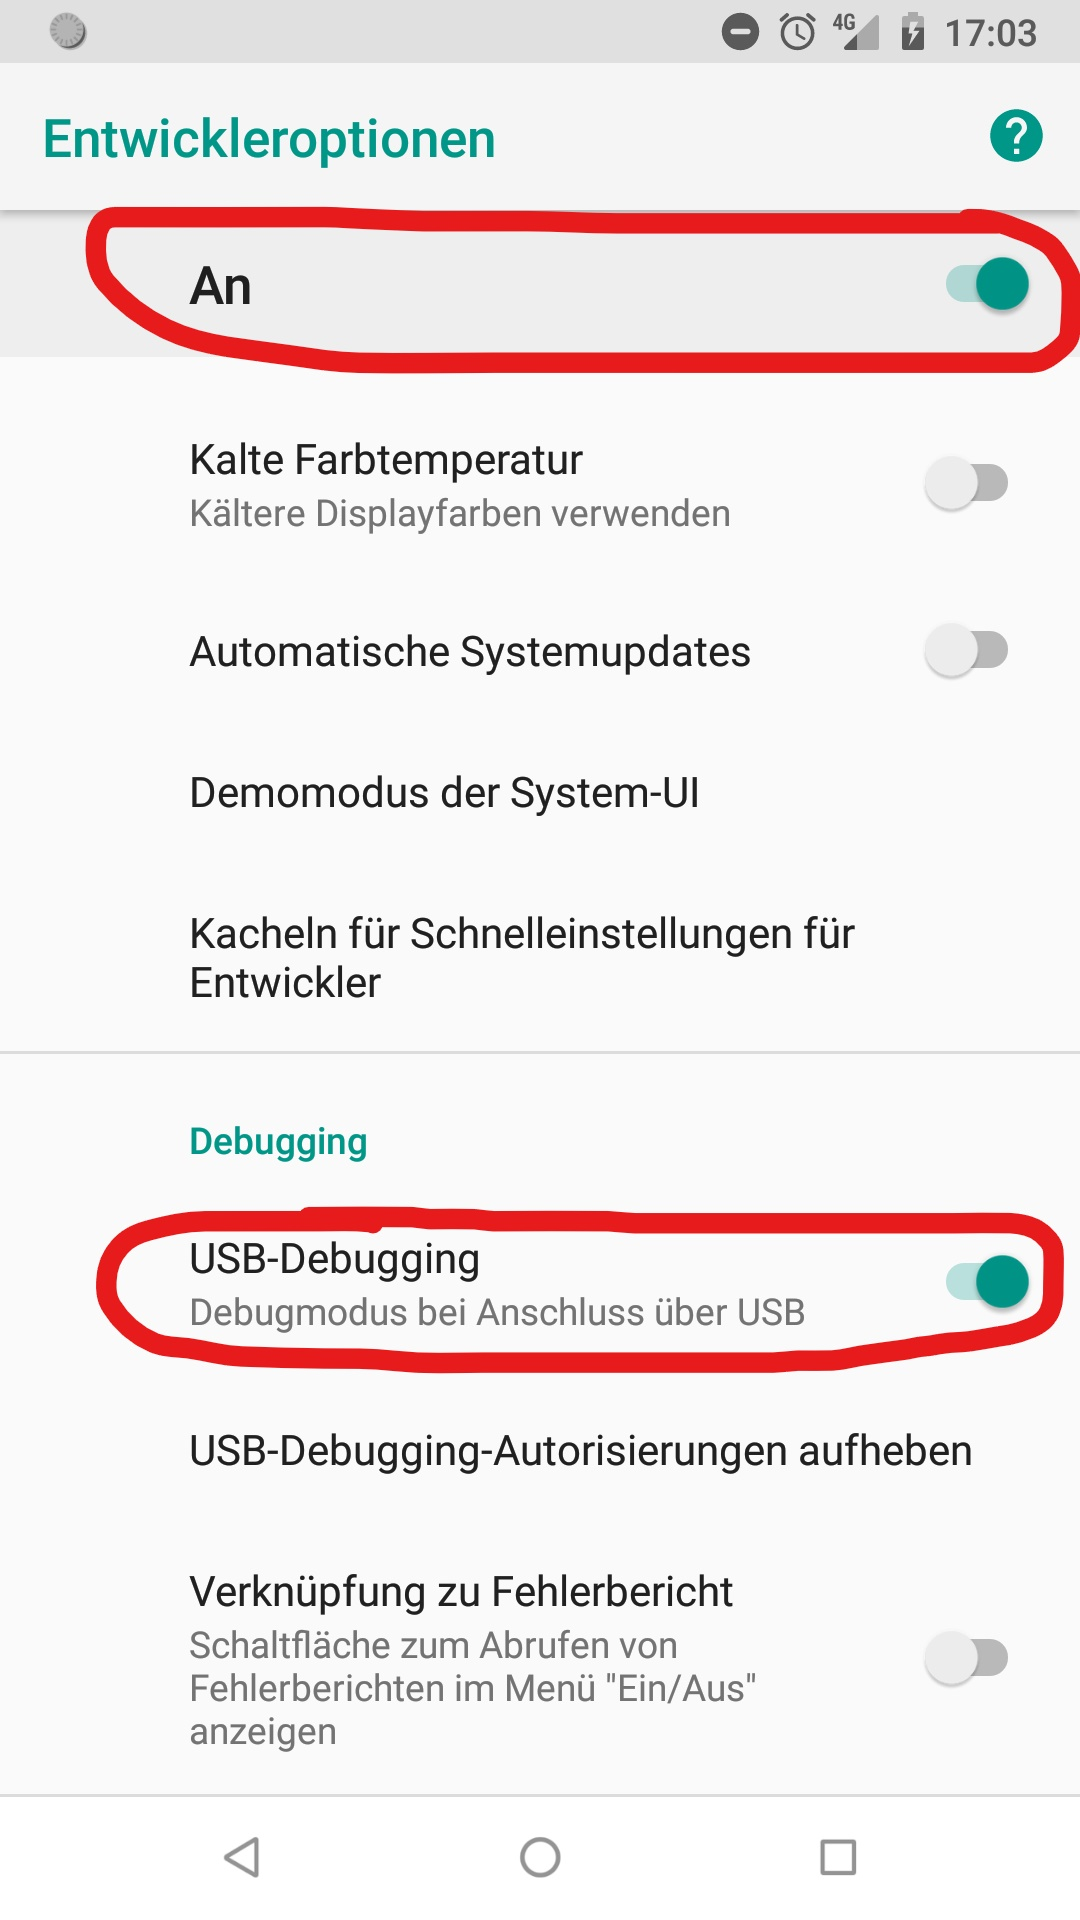
\includegraphics[width=6cm]{BilderAllgemein/DevToolsAndroid}\medskip
	\caption{Aktivieren der Entwicklertools auf Android 8.1.0}
	\label{fig:DevToolsAndorid}
\end{figure}

\begin{figure}[h]
	\centering
	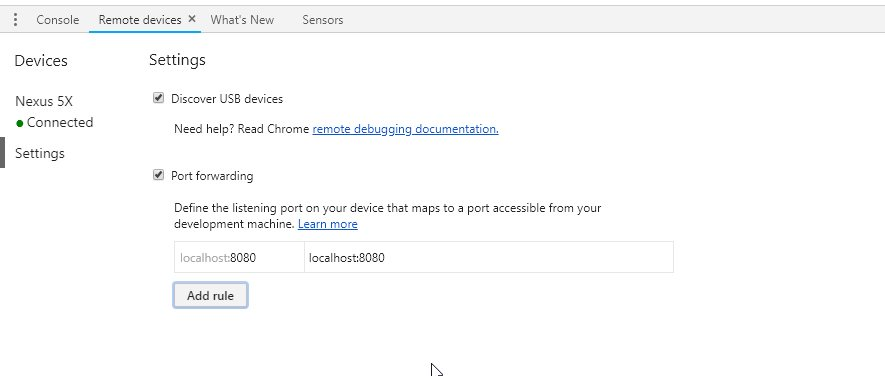
\includegraphics[width=14cm]{BilderAllgemein/DevToolsChrome}\medskip
	\caption{Anzeige der Verbindung auf Google Chrome 67}
	\label{fig:DevToolsChrome}
\end{figure}
\newpage
Falls kein Android Gerät zur Verfügung steht ist der von Android Studio\footnote{https://developer.android.com/studio/} angebotene Emulator eine große Hilfe. Durch den integrierten Emulator lassen sich verschiedene Softwareversionen von Android darstellen. Sie helfen bei der Entwicklung und beim Testen der \acs{PWA}.

\section{Lighthouse}
Lighthouse ist ein open-source Tool von Google und unterstützt den Entwickler bei der Verbesserung und Transformation der Applikation zu einer vollwertigen \acs{PWA}. Man kann Lighthouse über 3 Wege verwenden:
\begin{itemize}
    \item  in Chrome DevTools
	\item  über die Kommandozeile
	\item  oder im Continues Integration Prozess als Node Module
\end{itemize}
Jeder dieser Workflows benötigt den Google Chrome Browser \cite{Lighthouse}.
Der Einsatz von Lighthouse über den Browser ist einfach. Nach eingabe der URL kann das Tool über das Chrome PlugIn, wie in Abbildung \ref{fig:LighthousePlugIN} zu sehen ist, gestartet werden. Lighthouse führt einen Debuggingtest (Abbildung \ref{fig:LighthouseDebugging}) aus und erstellt einen Bericht. In Abbildung \ref{fig:LightH_beforHTTPS_Overview} ist der Überblick der Applikation zu sehen und in Abbildung \ref{fig:PWA_Test_Lighthouse_noHTTPS} werden die fehlenden PWA-Features angezeigt.

\begin{figure}[h]
	\centering
	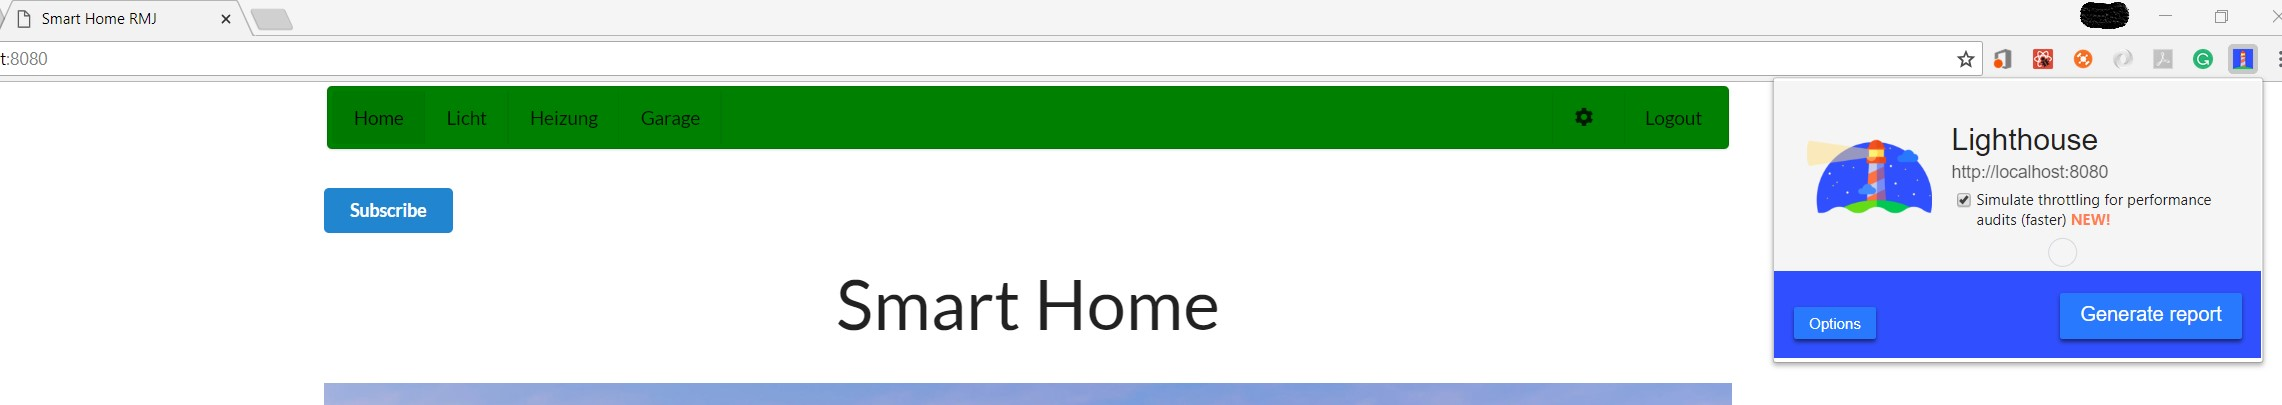
\includegraphics[width=8cm]{BilderAllgemein/Test/LighthousePlugIN}\medskip
	\caption{Lighthouse Plugin Chrome 67 }
	\label{fig:LighthousePlugIN}
\end{figure}

\begin{figure}[h]
	\centering
	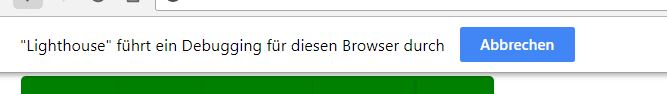
\includegraphics[width=8cm]{BilderAllgemein/Test/debuggingLighthouse}\medskip
	\caption{Debugging}
	\label{fig:LighthouseDebugging}
\end{figure}
 

\begin{figure}[H]
	\centering
	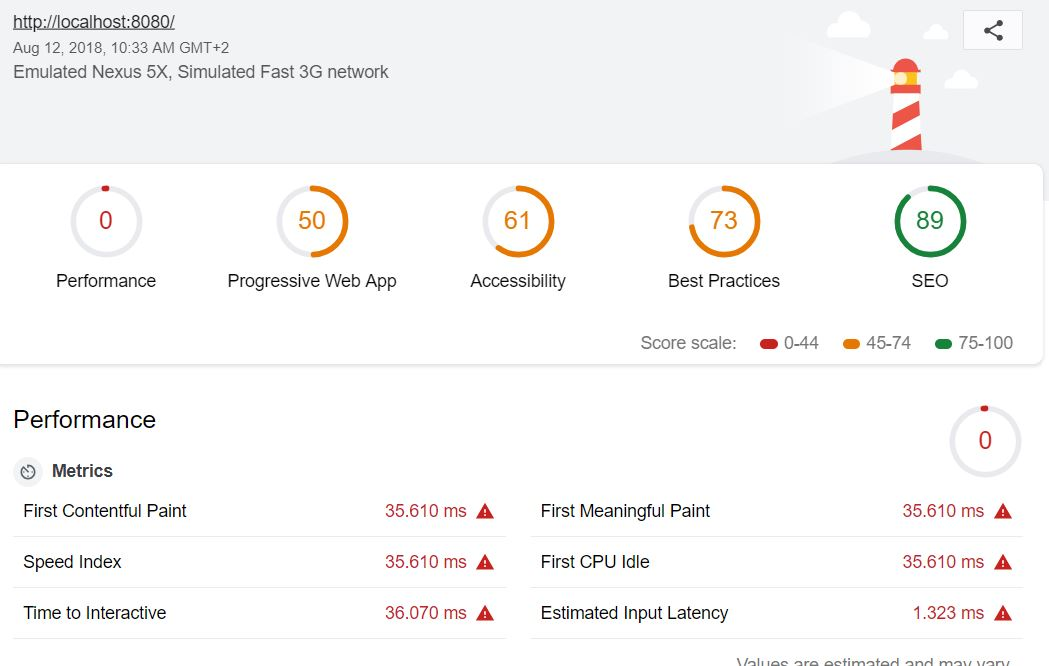
\includegraphics[width=10cm]{BilderAllgemein/Test/LightH_beforHTTPS_Overview}\medskip
	\caption{Lighthouse Überblick}
	\label{fig:LightH_beforHTTPS_Overview}
\end{figure}

\begin{figure}[h]
	\centering
	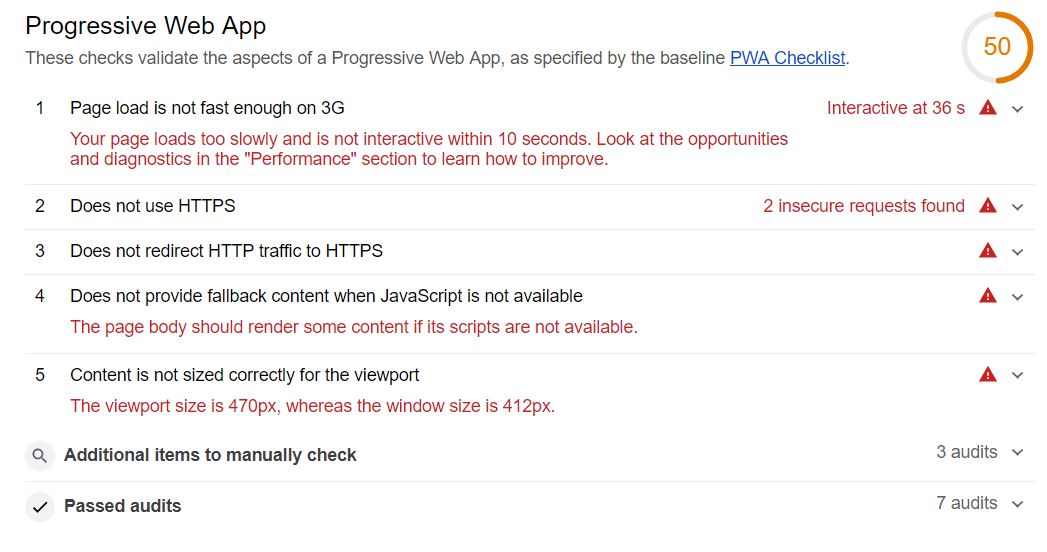
\includegraphics[width=10cm]{BilderAllgemein/Test/PWA_Test_Lighthouse_noHTTPS}\medskip
	\caption{Lighthouse fehlende PWA-Features}
	\label{fig:PWA_Test_Lighthouse_noHTTPS}
\end{figure}

In beiden Bericht Abbildungen \ref{fig:LightH_beforHTTPS_Overview} und \ref{fig:PWA_Test_Lighthouse_noHTTPS} erkennt man, dass die Applikation nur zur Hälfte die PWA Features enthält.
Dies kommt daher, weil die \acs{PWA} bei diesem Test auf auf dem Localhost läuft und nicht wie von Google gefordert über das HTTPS-Protokoll.
Das Projekt wurde für diese Arbeit nicht Live gestellt.


\section{Add to Homescreen}
%https://developers.google.com/web/fundamentals/app-install-banners/#test
Durch dieses Feature sollte die \acs{PWA} dem Benutzer das Gefühl einer Nativen App geben. Doch leider funktioniert diese Funktion nicht immer wie sie sollte.
Das Feature ist zurzeit nur auf Android und Chrome Browsern verfügbar und ist damit weit entfernt von den Native Apps. Startet oft nicht automatisch, ist aber durch das Menu aufrufbar wie in Abbildung \ref{fig:ADDHome} zu sehen ist.

\begin{figure}[h]
	\centering
	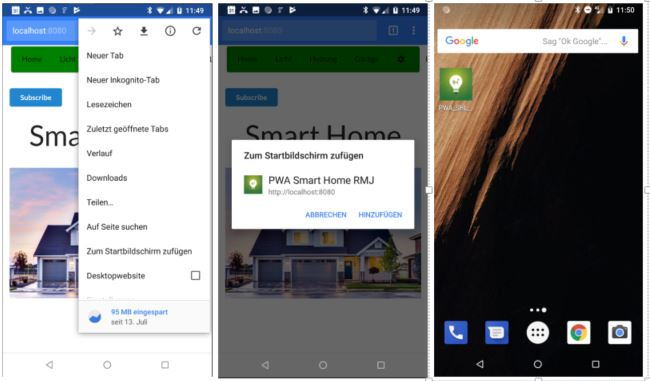
\includegraphics[width=10cm]{BilderAllgemein/Test/ADDHome}\medskip
	\caption{Add to Homescreen}
	\label{fig:ADDHome}
\end{figure}
\newpage

\section{Service Worker}
Die Status des Service Workers wird durch die DevTools geprüft.
Wie in Abbildung \ref{fig:SWTest} gezeigt ist pro \acs{PWA} nur ein Service Worker aktiv bei drei offenen Tabs. 

\begin{figure}[h]
	\centering
	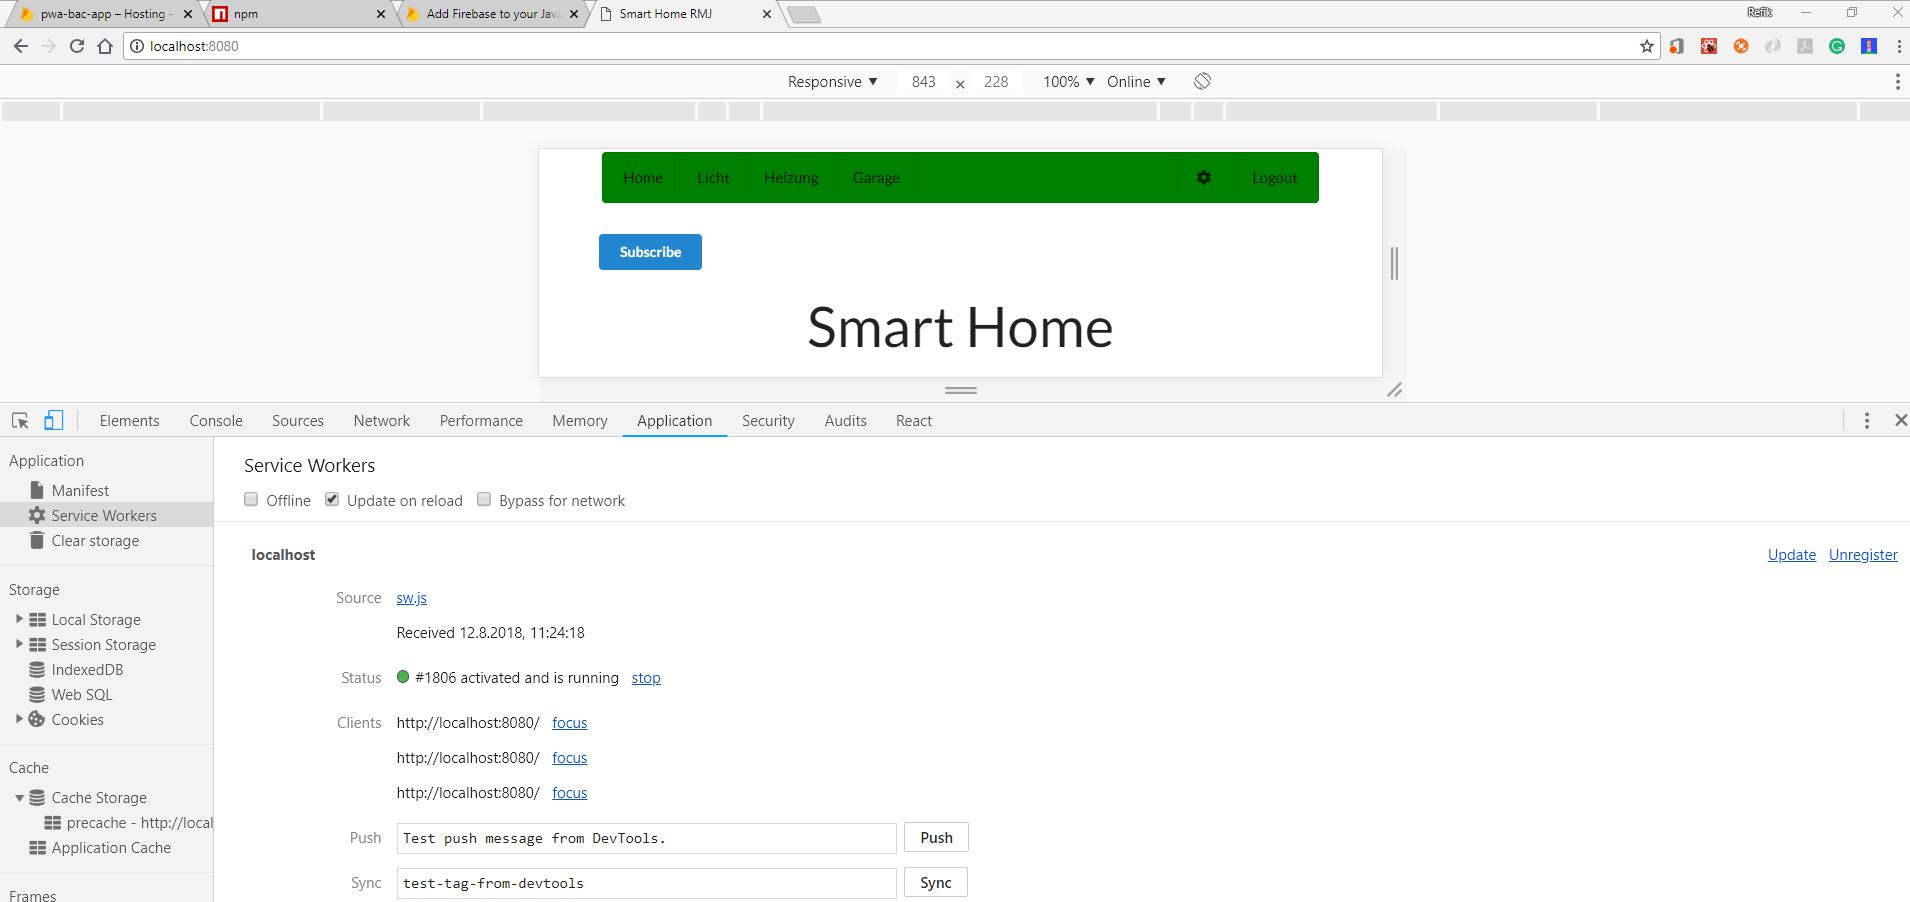
\includegraphics[width=10cm]{BilderAllgemein/Test/SW}\medskip
	\caption{Service Worker Status}
	\label{fig:SWTest}
\end{figure}
Weiters wurde die Offline Funktion der App getestet.
Abbildung \ref{fig:Offline} zeigt, dass die Applikation offline funktioniert.

\begin{figure}[h]
	\centering
	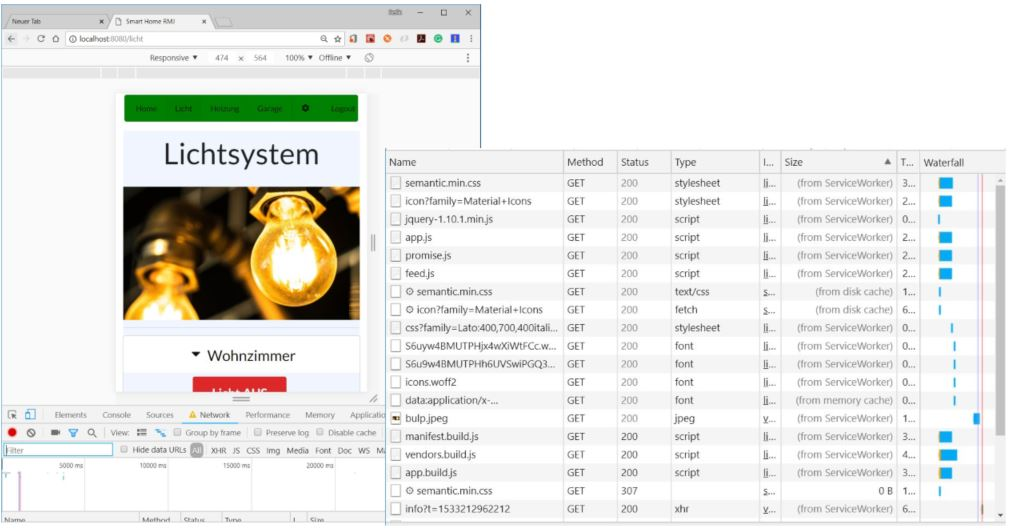
\includegraphics[width=14cm]{BilderAllgemein/Offline}\medskip
	\caption{Offline}
	\label{fig:Offline}
\end{figure}

\newpage

\section{Push Notifikation}
Um die Nachrichten erhalten zu können wird die Berechtigung (Abbildung \ref{fig:Registrierung}) als Erstes abgefragt und dann werden die Benachrichtigungen an den User erst verschickt siehe Abbildung \ref{fig:PushNotification}.

\begin{figure}[h]
	\centering
	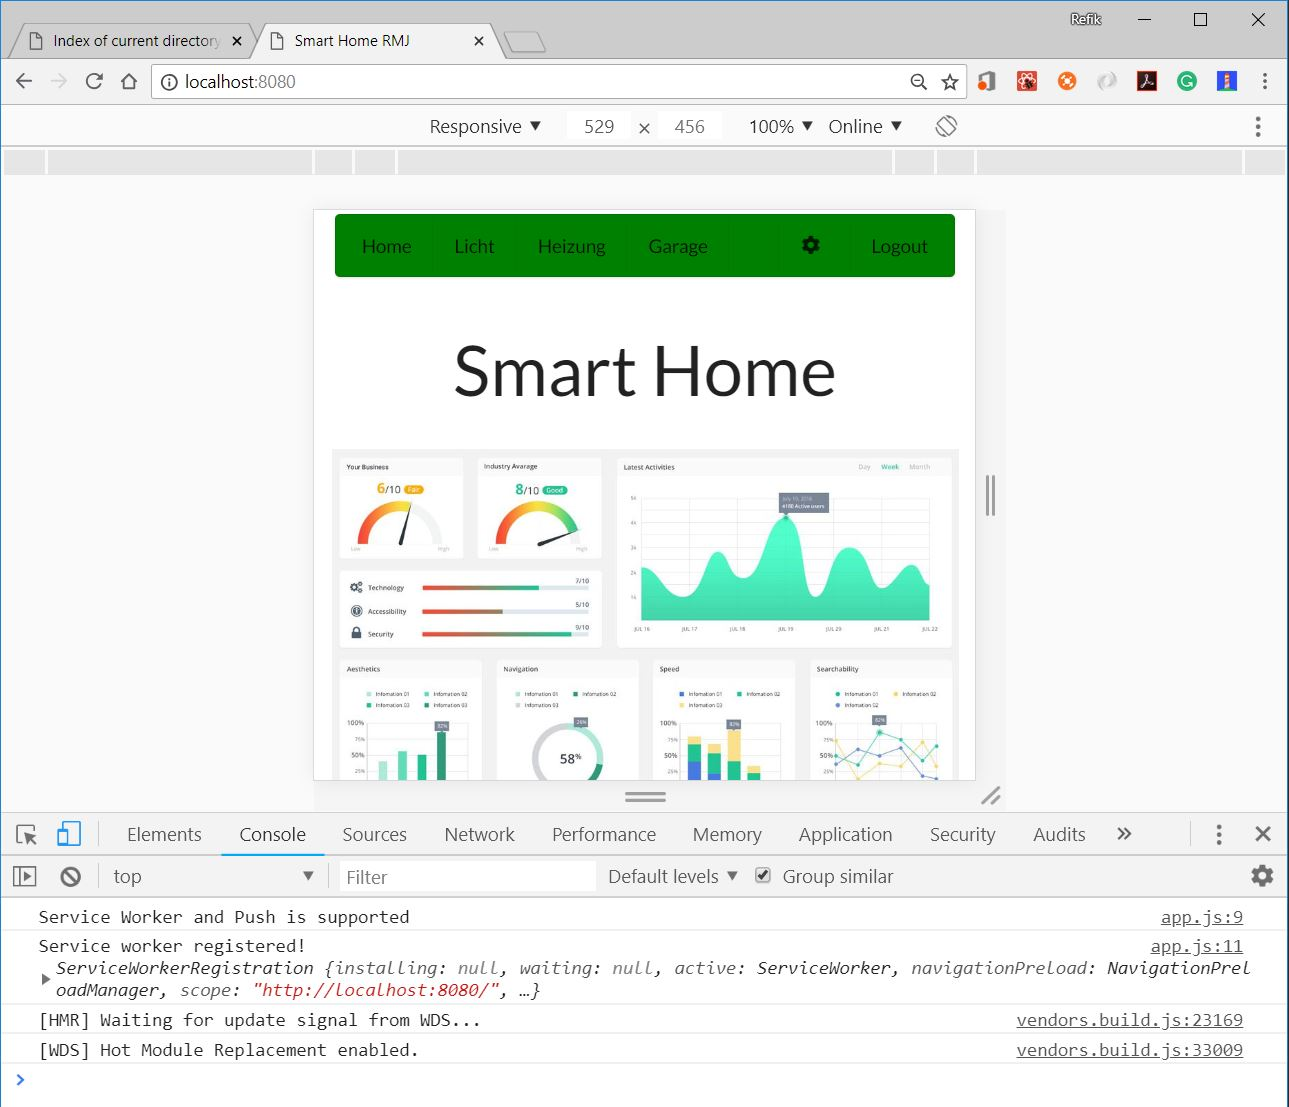
\includegraphics[width=10cm]{BilderAllgemein/PushNotification/Registrierung}\medskip
	\caption{Registrierung Push Notification}
	\label{fig:Registrierung}
\end{figure}

\begin{figure}[h]
	\centering
	
\includegraphics[width=14cm]{BilderAllgemein/PushNotification/Nachricht}\medskip
	\caption{Push Notification}
	\label{fig:Nachricht}
\end{figure}
\newpage

\section{Geolocation}
Die Geolocation Funktion muss den Nutzer immer fragen ob dieser seinen Standort bestimmt haben will. Wie in Abbildung \ref{fig:Registrierung} zu sehen ist, wird das in dem Prototypen umgesetzt. In der Abbildung \ref{fig:Maps} sieht man wie der Standort über die Geolocation-API ermittelt worden ist.

\begin{figure}[h]
	\centering
	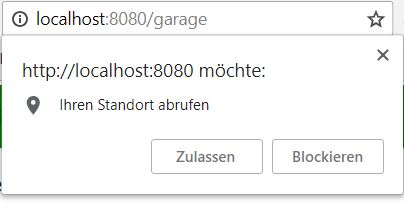
\includegraphics[width=10cm]{BilderAllgemein/Geolocation/Registrierung}\medskip
	\caption{Registrierung Geolocation}
	\label{fig:Registrierung}
\end{figure}

\begin{figure}[h]
	\centering
	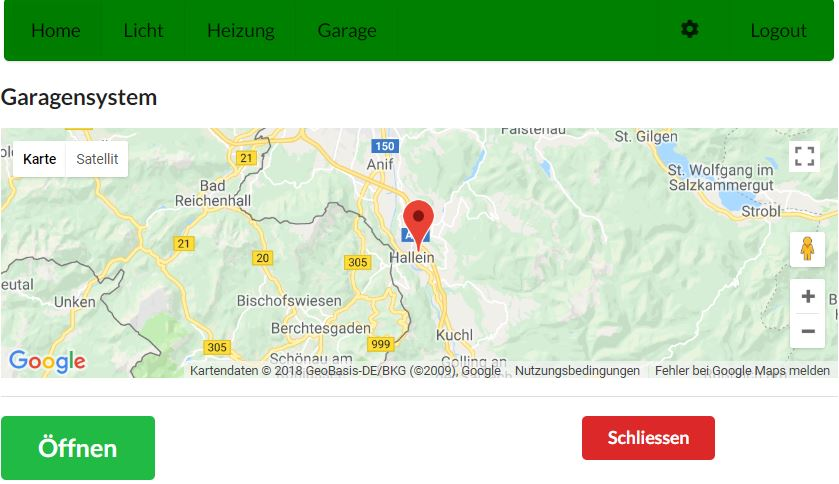
\includegraphics[width=14cm]{BilderAllgemein/Geolocation/Maps}\medskip
	\caption{Standortermittlung}
	\label{fig:Maps}
\end{figure}

\newpage
\section{Vergleich mit native App}
Im Vergleich zur Nativen App bietet die \acs{PWA} einige Vorteile aber auch Nachteile. Sie sind responsive, müssen nicht runtergeladen oder installiert werden und können zudem auf Geräte-API zugreifen und durch die Möglichkeit benachrichtigt zu werden wenn sich was ändert auch ein gute Alternative zu den native Apps.
Dank des Serviceworkers findet sich auch die Möglichkeit auch Applikation Offline zu betreiben oder bei niedriger Datenrate. Der Home Screen Banner verkürzt den Zugriff wesentlich .  
Durch die Entwicklung der \acs{PWA} pushed Google die verschlüsselte versenden der Nachrichten über das HTTPS-Protokoll.
Es sind aber auch noch einige Nachteile vorhanden, z.B.: funktionieren die oben genannten Features derzeit mehrheitlich nur am Androidgerät und dadurch ist diese Technologie nicht komplett Programmunabhängig.
Die Browser unterstützen auch noch nicht alles, insbesondere hinkt der Internet Explorer von Microsoft hinterher, dass ist deshalb ein Problem da Unternehmen noch auf diesen Browser setzten. 
Durch diese Tatsache ist die Native App für eine Angepasste Anwendung die bessere Wahl, aber was sicherlich vorstellbar ist, das die Technologie sich bei temporären Benötigten Webseiten oder Nachrichtendienstseiten durchsetzten kann.
Die \acs{PWA} wird die Native Apps wahrscheinlich nie ersetzten, aber sie haben sicher das Potenzial eine feste Strategie bei der Entwicklung von \acs{Web-App}s zu werden.



